\hypertarget{part-1-design-3}{
\section{Part 1, design 3}\label{part-1-design-3}}

\begin{figure}[ht]
  \centering
  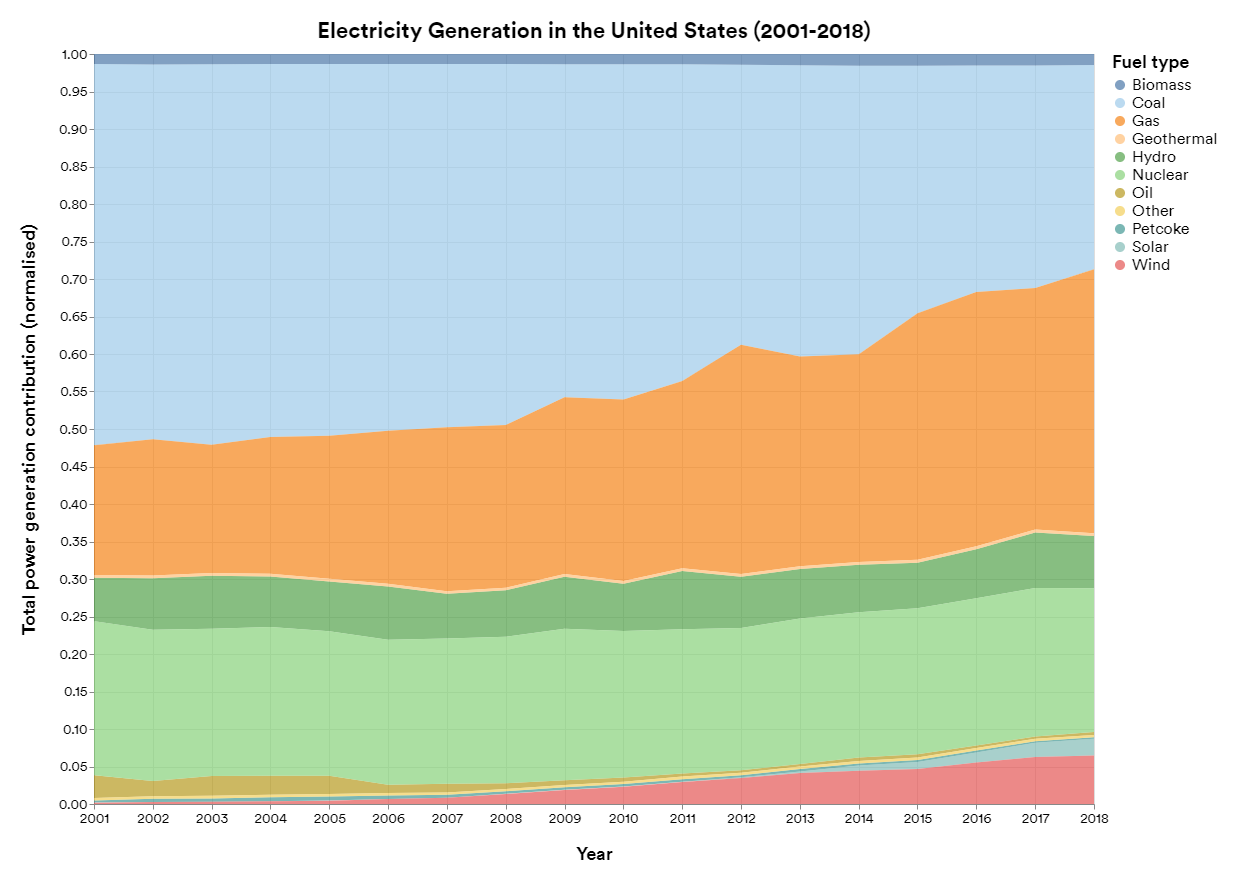
\includegraphics[width=\textwidth]{../img/design3}
  \caption{Electricity generation in the United States (Design 3)}
\end{figure}

\hypertarget{description}{
\subsubsection{Description}\label{description}}

\begin{description}
\item[Visual Design Type:]
Area chart
\item[Name of Tool:]
Altair
\item[Country:]
United States
\item[Year:]
2001-2018

\item[Visual Mappings:]
% each of the visual design mappings; include the data apping information about colour, shape, size, position (x/y axes), and any other visual mappings 
\begin{itemize}
  \item \textbf{Area}: Power generation contribution for each fuel type is shown by the area occupied by each stacked band of colour. At any given year, the bands combine to 100 percent of power generated.
  \item \textbf{Hue}: Fuel type is distinguished using a categorical hue scale.
\end{itemize}

\item[Unique Observation:]
% things we can learn from the visualisation e.g. from this vis we can see this pattern
This chart illustrates how electricity production in the US has evolved over an 18-year period. It is not concerned with actual production amounts, instead showing a normalised percentage contribution of each fuel type to the total power generation. Unnormalised charts may deceive users as changes in production of one fuel type can appear to have cascading effects on others.

We can then see clearly that renewable sources, especially wind and solar have slowly risen from almost nothing - whereas oil has largely died out. Whilst nuclear power remains largely the same, gas has overtaken coal as the dominant fuel type - presumably as the United States look to reduce their energy emissions.

\item[Data Preparation:]
% any modifications to the original data that had to be performed to generate your beautiful image
The provided GPPD data set was combined with a second which detailed electricity generation in the US by fuel type, dating back to 2001. Generation data was aggregated by year, then normalised in order to determine percentage contribution of each fuel source rather than amount produced.

\end{description}

% Describe the insight that your visualizations provide. What can we learn from
% your visualizations? How are they better than a standard line, pie, or bar
% chart?